
\documentclass{beamer}
\usepackage[utf8]{inputenc}
\usepackage[brazil]{babel}
\usepackage{graphicx}
\inputencoding{latin1}
\usetheme{metropolis}           % Use metropolis theme
\title{Uma Abordagem Colaborativa para o Gerenciamento de Dados em IoT}
\date{\today}
\author{J\^{o}natas Ribeiro Senna Pires}
\institute{Univesidade de Bras\'{i}lia}
\begin{document}

  \maketitle

  \begin{frame}{Outline}
    \setbeamertemplate{section in toc}[sections numbered]
    \tableofcontents[hideallsubsections]
  \end{frame}

\section{Sobre o Trabalho}
\begin{frame}{Sobre o Trabalho}
  Um sistema colaborativo para avalia\c{c}\~{a}o e classifica\c{c}\~{a}o de qualidade de dados gerados por sensores em um ambiente Internet das Coisas.
\end{frame}

  \section{Objetivos}
  \begin{frame}{Objetivos}
    \begin{itemize}
        \item Implantar uma rede de sensores conectados \`{a} Internet;
        \item Montar um servidor para o armazenamento de dados e realiza\c{c}\~{a}o da aplica\c{c}\~{a}o;
        \item Desenvolver um m\'{o}dulo de distribui\c{c}\~{a}o de tarefas;
        \item Desenvolver um m\'{o}dulo de avalia\c{c}\~{a}o e classifica\c{c}\~{a}o de qualidade;
        \item Desenvolver uma interface gr\'{a}fica para o acesso das informa\c{c}\~{o}es geradas pelo sistema.
    \end{itemize}
  \end{frame}

  \section{Sensores}
  \begin{frame}{Montagem}
    \begin{center}
    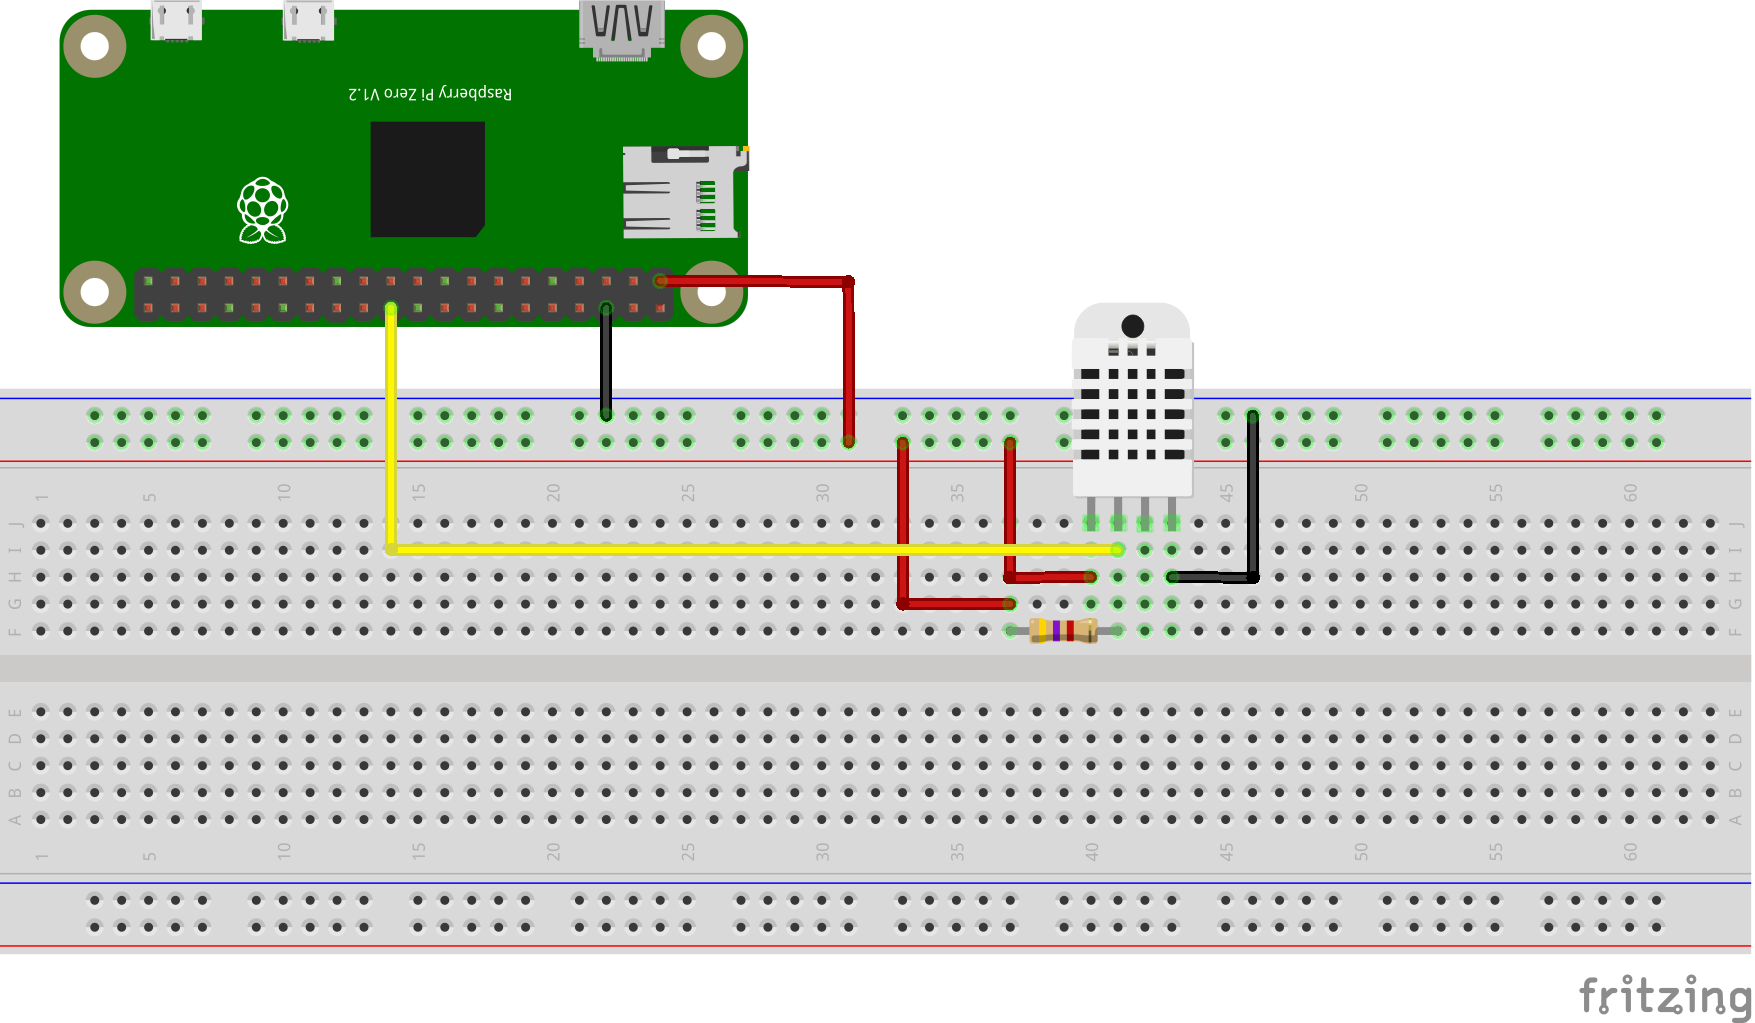
\includegraphics[height=130pt, width=175pt]{sensor}
  \end{center}
    \begin{itemize}
      \item Raspberry Pi Zero W;
      \item Sensor DHT 11;
    \end{itemize}
  \end{frame}
  \begin{frame}{Comunica\c{c}\~{a}o}
    %\includegraphics[height=200pt, width=325pt]{CBafesDER2}
    \begin{itemize}
      \item Mensagens no formato JSON;
      \item Envio de dados a cada cinco minutos;
      \item Bibliotecas json e requests para Python para comunica\c{c}\~{a}o entre sensor-servidor.
    \end{itemize}
  \end{frame}
  \begin{frame}{Escalabilidade}
    A primeira mensagem enviada ao servidor \'{e} a mais completa, com informa\c{c}\~{o}es de localiza\c{c}\~{a}o do sensor e os valores de identifica\c{c}\~{a}o nulos. Ao receber esta primeira mensagem, o servidor identifica que \'{e} um novo sensor, lhe atribui um ID e envia uma resposta com o valor do identificador. A partir desse momento as pr\'{o}ximas mensagens ser\~{a}o compostas apenas dos valores medidos, data, hor\'{a}rio e identificador.
  \end{frame}


  \section{Ferramentas Utilizadas}
  \begin{frame}{Ferramentas Utilizadas}
    \\\textbf{SGBDs Utilizados}
    \begin{itemize}
      \item PostgreSQL;
      \item SQLite.
    \end{itemize}
    \\\textbf{Linguagens Utilizadas}
        \begin{itemize}
            \item Python;
            \item Python(framework Django), HTML e CSS.
        \end{itemize}
  \end{frame}

  \section{Resultados Parciais}
  \begin{frame}{ Resultados }
        \begin{itemize}
            \item A rede de sensores foi implantada;
            \item A aquisi\c{c}\~ao de dados funciona da maneira esperada (1 GB at\'{e} agora);
            \item Progressos no sistema de atribui\c{c}\~ao de tarefas ao sensor.
        \end{itemize}
  \end{frame}

  \section{Problemas Encontrados}
  \begin{frame}{Problemas}
        \begin{itemize}
            \item Gera\c{c}\~ao de QR codes para identifica\c{c}\~ao do sensor e redirecionamento para a p\'agina com as tarefas;
            \item Interface gr\'afica.
        \end{itemize}
  \end{frame}

  \section{Continua\c{c}\~ao do Trabalho}
  \begin{frame}{Continua\c{c}\~ao do Trabalho}
        \begin{itemize}
            \item Implementar a distribui\c{c}\~ao de tarefas;
            \item Implementar o m\'odulo de avalia\c{c}\~ao e classifica\c{c}\~ao;
            \item Implementar a interface gr\'afica.
        \end{itemize}
  \end{frame}
  \begin{frame}
    \begin{center}
  Obrigado!
\end{center}

  \end{frame}
\end{document}
